\documentclass[12pt,a4paper]{article}

% ── Packages ──────────────────────────────────────────────────────────────────
\usepackage[a4paper, margin=2.5cm, headheight=15pt]{geometry}
\usepackage{fontenc}
\usepackage{inputenc}
\usepackage{microtype}
\usepackage{parskip}
\usepackage{setspace}
\usepackage{titlesec}
\usepackage{hyperref}
\usepackage{xcolor}
\usepackage{graphicx}
\usepackage{booktabs}
\usepackage{tabularx}
\usepackage{array}
\usepackage{longtable}
\usepackage{enumitem}
\usepackage{fancyhdr}
\usepackage{amsmath}
\usepackage{amssymb}
\usepackage{listings}
\usepackage{mdframed}
\usepackage{tcolorbox}
\usepackage{pifont}
\usepackage{caption}

\tcbuselibrary{breakable}

% ── Colours ───────────────────────────────────────────────────────────────────
\definecolor{darkblue}{RGB}{13,71,161}
\definecolor{accentblue}{RGB}{25,118,210}
\definecolor{lightgray}{RGB}{245,245,245}
\definecolor{codegray}{RGB}{248,248,248}
\definecolor{bordergray}{RGB}{200,200,200}
\definecolor{darkgreen}{RGB}{27,94,32}
\definecolor{darkred}{RGB}{183,28,28}
\definecolor{quotebg}{RGB}{232,244,253}
\definecolor{quoteborder}{RGB}{25,118,210}
\definecolor{ragbg}{RGB}{224,242,241}
\definecolor{ragborder}{RGB}{0,105,92}
\definecolor{plainbg}{RGB}{237,231,246}
\definecolor{plainborder}{RGB}{81,45,168}

% ── Hyperref setup ────────────────────────────────────────────────────────────
\hypersetup{
    colorlinks=true,
    linkcolor=darkblue,
    urlcolor=accentblue,
    citecolor=darkblue,
    pdftitle={Knowledge Graph-Augmented RAG System for Adaptive Learning},
    pdfauthor={Aaditya Bhatia, Aryan Chaudhary},
}

% ── Section formatting ────────────────────────────────────────────────────────
\titleformat{\section}
  {\Large\bfseries\color{darkblue}}
  {\thesection}{1em}{}[\vspace{2pt}\titlerule]

\titleformat{\subsection}
  {\large\bfseries\color{accentblue}}
  {\thesubsection}{1em}{}

\titleformat{\subsubsection}
  {\normalsize\bfseries}
  {\thesubsubsection}{1em}{}

\titlespacing*{\section}{0pt}{20pt}{8pt}
\titlespacing*{\subsection}{0pt}{14pt}{4pt}
\titlespacing*{\subsubsection}{0pt}{10pt}{3pt}

% ── Header / Footer ───────────────────────────────────────────────────────────
\pagestyle{fancy}
\fancyhf{}
\fancyhead[L]{\small\color{gray}Knowledge Graph-Augmented RAG --- AoLM}
\fancyhead[R]{\small\color{gray}CLD Duos}
\fancyfoot[C]{\small\thepage}
\renewcommand{\headrulewidth}{0.4pt}

% ── Code listing style ────────────────────────────────────────────────────────
\lstdefinestyle{codestyle}{
  backgroundcolor=\color{codegray},
  basicstyle=\ttfamily\footnotesize,
  breakatwhitespace=false,
  breaklines=true,
  captionpos=b,
  commentstyle=\color{darkgreen},
  keywordstyle=\color{darkblue}\bfseries,
  stringstyle=\color{darkred},
  frame=single,
  rulecolor=\color{bordergray},
  framesep=4pt,
  xleftmargin=8pt,
  xrightmargin=4pt,
  numbers=none,
  showstringspaces=false,
  tabsize=2,
  columns=flexible,
}
\lstset{style=codestyle}

% ── Quote box (blockquote) ────────────────────────────────────────────────────
\newenvironment{quotebox}{%
  \begin{tcolorbox}[
    colback=quotebg,
    colframe=quoteborder,
    left=6pt, right=6pt, top=4pt, bottom=4pt,
    boxrule=0.5pt,
    leftrule=3pt,
    arc=2pt,
    breakable,
  ]
  \itshape\small
}{%
  \end{tcolorbox}
}

% ── RAG response box ──────────────────────────────────────────────────────────
\newenvironment{ragbox}[1]{%
  \begin{tcolorbox}[
    title={\textbf{#1}},
    colback=ragbg,
    colframe=ragborder,
    colbacktitle=ragborder,
    coltitle=white,
    left=6pt, right=6pt, top=4pt, bottom=4pt,
    boxrule=0.5pt,
    arc=3pt,
    fonttitle=\small\bfseries,
    breakable,
  ]
  \small
}{%
  \end{tcolorbox}
}

% ── Plain response box ────────────────────────────────────────────────────────
\newenvironment{plainbox}[1]{%
  \begin{tcolorbox}[
    title={\textbf{#1}},
    colback=plainbg,
    colframe=plainborder,
    colbacktitle=plainborder,
    coltitle=white,
    left=6pt, right=6pt, top=4pt, bottom=4pt,
    boxrule=0.5pt,
    arc=3pt,
    fonttitle=\small\bfseries,
    breakable,
  ]
  \small
}{%
  \end{tcolorbox}
}

% ── Helpers ───────────────────────────────────────────────────────────────────
\newcommand{\tick}{\textcolor{darkgreen}{\ding{51}}}
\newcommand{\cross}{\textcolor{darkred}{\ding{55}}}

\setlength{\parskip}{6pt}
\setlength{\parindent}{0pt}
\onehalfspacing

% ══════════════════════════════════════════════════════════════════════════════
\begin{document}
% ══════════════════════════════════════════════════════════════════════════════

% ── Title page ────────────────────────────────────────────────────────────────
\begin{titlepage}
  \thispagestyle{empty}
  \centering
  \vspace*{3cm}

  {\Huge\bfseries\color{darkblue}
    Knowledge Graph-Augmented RAG System\\[6pt]
    for Adaptive DSA Learning
  \par}

  \vspace{1.5cm}
  \rule{0.6\textwidth}{1pt}
  \vspace{1.2cm}

  {\large
    \textbf{Course:} Application of Language Modeling (AoLM)\\[8pt]
    \textbf{Team:} CLD Duos\\[8pt]
    \textbf{Members:}\\[6pt]
    Aaditya Bhatia \quad (2023114012)\\[4pt]
    Aryan Chaudhary \quad (2023114015)
  \par}

  \vspace{1.2cm}
  \rule{0.6\textwidth}{1pt}

  \vfill
\end{titlepage}

% ── Table of Contents ─────────────────────────────────────────────────────────
\thispagestyle{empty}
\tableofcontents
\clearpage

% ══════════════════════════════════════════════════════════════════════════════
\section{Overview}
% ══════════════════════════════════════════════════════════════════════════════

This project builds an \textbf{Adaptive Learning System} for Data Structures
and Algorithms (DSA) by combining two technologies: a \textbf{Knowledge Graph
(KG)} extracted from the CLRS textbook and a \textbf{Large Language Model
(LLM)} running locally. The core idea is that a plain LLM, while knowledgeable,
has no awareness of \textit{who} is asking or \textit{what} they already know.
By grounding the LLM in a structured KG that encodes prerequisites, concept
relationships, and common misconceptions, the system can personalise its
explanations to each learner.

The pipeline works in two phases:

\begin{enumerate}
  \item \textbf{Offline Phase (KG Construction):} The CLRS textbook is parsed,
    chunked semantically, and each chunk is processed by Google Gemini 2.5 Pro
    to extract concepts, relationships, and misconceptions into a Neo4j graph
    database.

  \item \textbf{Online Phase (RAG Inference):} When a student asks a question,
    the KG is queried for the relevant concept's context (prerequisites,
    subtypes, misconceptions, what it unlocks), this context is injected into
    the LLM prompt alongside the student's profile, and Qwen 2.5 7B generates a
    tailored response.
\end{enumerate}

% ══════════════════════════════════════════════════════════════════════════════
\section{Knowledge Graph Construction}
% ══════════════════════════════════════════════════════════════════════════════

\subsection{Source Material}

The source textbook is:

\begin{tcolorbox}[colback=lightgray, colframe=bordergray, arc=3pt,
  left=10pt, right=10pt, top=6pt, bottom=6pt]
  \textbf{Introduction to Algorithms, 3rd Edition}\\
  Thomas H.\ Cormen, Charles E.\ Leiserson, Ronald L.\ Rivest, Clifford Stein\\
  MIT Press --- commonly referred to as \textbf{CLRS}
\end{tcolorbox}

CLRS is the gold standard reference for algorithms and data structures, used in
universities worldwide. It is a 1,313-page book covering sorting, graph
algorithms, dynamic programming, data structures, number-theoretic algorithms,
and much more. It was chosen because:

\begin{itemize}
  \item It is highly structured with numbered chapters and sections
    (e.g., \texttt{13.3 Insertion into a red-black tree})
  \item It explicitly discusses prerequisites, properties, and common pitfalls
  \item Its depth makes it an ideal source for a pedagogical KG
\end{itemize}

\subsection{PDF Parsing and Semantic Chunking}

The PDF is parsed using \textbf{PyMuPDF (fitz)}, which extracts text
block-by-block, preserving the reading order of each page. A naive full-text
split would lose section boundaries, so a \textbf{semantic chunking} approach
was used instead.

CLRS section headings follow a consistent pattern, for example:

\begin{lstlisting}
1  The Role of Algorithms in Computing
1.1  Algorithms
Chapter 13  Red-Black Trees
13.1  Properties of red-black trees
\end{lstlisting}

This pattern is captured with the following regular expression:

\begin{lstlisting}[language=Python]
HEADING_RE = re.compile(
    r"^(?:Chapter\s+)?\d+(?:\.\d+)*\s{2,}.+$",
    re.MULTILINE,
)
\end{lstlisting}

The full text is split on every matched heading, producing one chunk per
section. Sections longer than \textbf{4,000 characters} ($\approx$1,000 tokens)
are further split on paragraph boundaries (\texttt{\textbackslash
n\textbackslash n}) to stay within token limits without cutting in the middle of
a concept. Chunks shorter than \textbf{100 characters} (e.g.,
table-of-contents entries and page-number lines) are filtered out before
processing.

\textbf{Result:} 1,018 meaningful semantic chunks from 1,313 pages.

\subsection{LLM-Based Entity and Relation Extraction}

Chunks are processed in \textbf{batches of 5} (approximately 20,000 characters
per batch) by \textbf{Google Gemini 2.5 Pro} via the \texttt{google-genai} SDK.
The REST transport (\texttt{api\_version="v1beta"}) was used instead of gRPC to
ensure stability on restricted networks.

The model was chosen for its:
\begin{itemize}
  \item \textbf{Superior reasoning ability} --- needed to infer implicit
    relationships
  \item \textbf{Large context window} --- handles multi-section batches
    comfortably
  \item \textbf{JSON output reliability} --- critical for structured extraction
\end{itemize}

\textbf{Rate limiting and retries:} Exponential backoff with up to 6 retries
was implemented to handle \texttt{429 RESOURCE\_EXHAUSTED} errors. A
\texttt{progress.json} file tracks the last successfully processed chunk,
allowing the pipeline to resume from where it left off after quota resets or
network failures.

\subsection{Extraction Prompt Design}

Each batch call sends the combined text of 5 sections with the following prompt:

\begin{lstlisting}
You are an expert Data Structures & Algorithms Curriculum Designer.
Analyse the following educational text from the CLRS textbook
"Introduction to Algorithms". It contains {N} sections.

TEXT TO ANALYSE:
"""
[Section: {title_1}]
{text_1}
---
[Section: {title_2}]
{text_2}  ...
"""

Identify three things across ALL sections:

1. CONCEPTS: Key technical terms
   Assign each a SHORT snake_case unique id.

2. RELATIONSHIPS between concepts:
   - "REQUIRES"   : A requires B as a prerequisite.
   - "SUBTYPE_OF" : A is a specialised type / variant of B.
   - "USES"       : A employs B as a technique or data structure.

3. MISCONCEPTIONS: Common mistakes explicitly mentioned or implied.

Rules:
- Only include items clearly supported by the provided text.
- Every concept id in relationships MUST appear in the concepts list.
- Return ONLY a raw JSON object -- no markdown fences, no extra text.
\end{lstlisting}

\textbf{Key design decisions in this prompt:}

\begin{itemize}
  \item \textbf{Role assignment} (``expert DSA curriculum designer'') --- steers
    Gemini towards pedagogical extraction rather than generic summarisation.
  \item \textbf{Three-category schema} --- separates factual concepts, structural
    relationships, and pedagogical misconceptions, which a plain summarisation
    prompt would conflate.
  \item \textbf{Strict JSON-only output rule} --- prevents markdown fencing or
    explanatory preamble that would break the JSON parser.
  \item \textbf{Section labels in the batch text} --- gives the model context
    about where each excerpt came from, helping it attribute relationships
    correctly.
  \item \textbf{Explicit relationship semantics} --- REQUIRES, SUBTYPE\_OF, and
    USES are defined clearly so the model does not conflate ``a specialisation''
    with ``a prerequisite.''
\end{itemize}

\subsection{Neo4j Ingestion}

The extracted JSON is pushed to a \textbf{Neo4j Aura} cloud instance using
idempotent \texttt{MERGE} statements, so the pipeline can safely re-run without
creating duplicate nodes. Three types of data are stored:

\begin{lstlisting}[language=SQL]
-- Concept nodes
MERGE (c:Concept {id: $id})
SET c.name = $name, c.definition = $definition

-- Dependency relationships
MATCH (a:Concept {id: $source}), (b:Concept {id: $target})
MERGE (a)-[:REQUIRES]->(b)
-- (similarly for SUBTYPE_OF and USES)

-- Misconception nodes linked to concepts
MERGE (m:Misconception {description: $desc})
MERGE (c:Concept {id: $cid})-[:HAS_MISCONCEPTION]->(m)
\end{lstlisting}

\subsection{Knowledge Graph Statistics}

After processing all 1,018 chunks across 204 API calls to Gemini 2.5 Pro, the
final KG contains:

\begin{center}
\begin{tabular}{lc}
  \toprule
  \textbf{Entity / Relationship} & \textbf{Count} \\
  \midrule
  Concept nodes              & \textbf{1,829} \\
  Misconception nodes        & \textbf{709}   \\
  USES relationships         & \textbf{1,072} \\
  HAS\_MISCONCEPTION         & \textbf{709}   \\
  REQUIRES relationships     & \textbf{648}   \\
  SUBTYPE\_OF relationships  & \textbf{508}   \\
  \midrule
  \textbf{Total relationships} & \textbf{2,937} \\
  \bottomrule
\end{tabular}
\end{center}

This means the KG captures not just \textit{what} the book says, but
\textit{how concepts connect to each other} --- forming a genuine dependency
graph that can drive adaptive tutoring.

% ══════════════════════════════════════════════════════════════════════════════
\section{Knowledge Graph Visualisation}
% ══════════════════════════════════════════════════════════════════════════════

The following visualisation shows a portion of the extracted Knowledge Graph,
rendered from Neo4j. Each node represents a concept from CLRS, and the directed
edges represent the three relationship types --- \textbf{REQUIRES} (prerequisite
dependency), \textbf{SUBTYPE\_OF} (taxonomic hierarchy), and \textbf{USES}
(algorithmic technique usage).

\begin{figure}[h!]
  \centering
  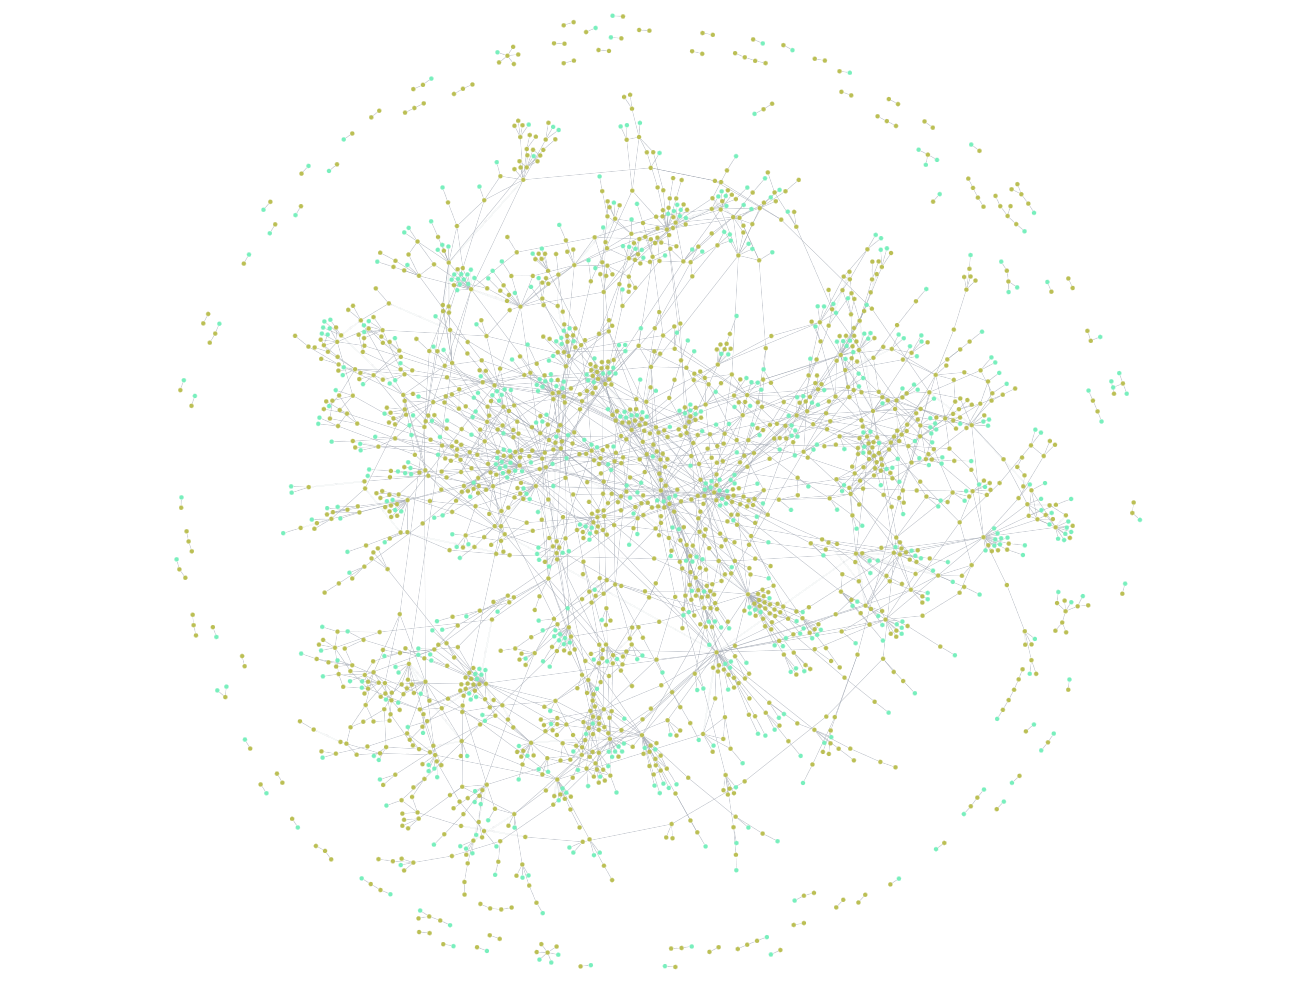
\includegraphics[width=\textwidth]{visualisation.png}
  \caption{Knowledge Graph extracted from the CLRS textbook (Neo4j Aura).
    Node clusters near the centre represent highly connected foundational
    concepts. Peripheral nodes are specialised topics with many incoming
    prerequisite edges.}
  \label{fig:kg}
\end{figure}

Nodes clustered in the centre represent highly interconnected foundational
concepts such as \textit{Binary Tree}, \textit{Graph}, \textit{Sorting}, and
\textit{Recursion} --- concepts that are prerequisites for a very large number
of other topics. Peripheral nodes represent more specialised topics like
\textit{Red-Black Tree Deletion} or \textit{Fibonacci Heap Decrease-Key} that
have many incoming prerequisite edges but few outgoing ones.

The \textbf{Misconception nodes} (not shown in this view for clarity) are
connected via \texttt{HAS\_MISCONCEPTION} edges and provide the RAG engine with
a curated list of common errors to proactively address in explanations.

% ══════════════════════════════════════════════════════════════════════════════
\section{RAG Engine Architecture}
% ══════════════════════════════════════════════════════════════════════════════

\subsection{Query and Context Building}

When a student asks a question about a topic (e.g., \texttt{"dijkstra"}), the
RAG engine queries Neo4j to retrieve:

\begin{enumerate}
  \item \textbf{Concept definition and section reference} from CLRS
  \item \textbf{Direct prerequisites} --- concepts that must be understood first
    (\texttt{REQUIRES} edges outgoing)
  \item \textbf{What this topic unlocks} --- concepts that build upon it
    (\texttt{REQUIRES} edges incoming)
  \item \textbf{Subtypes} --- variants and specialisations
    (\texttt{SUBTYPE\_OF} edges)
  \item \textbf{Techniques used} --- algorithms or structures it relies on
    (\texttt{USES} edges)
  \item \textbf{Misconceptions} --- common errors associated with this concept
    (\texttt{HAS\_MISCONCEPTION} edges)
\end{enumerate}

The matching is done using a \textbf{fuzzy \texttt{CONTAINS} match} in Cypher:

\begin{lstlisting}[language=SQL]
MATCH (c:Concept)
WHERE toLower(c.name) CONTAINS toLower($topic)
   OR toLower(c.id)   CONTAINS toLower($topic)
RETURN c.id, c.name, c.definition, c.section
LIMIT 5
\end{lstlisting}

This tolerates partial topic names and small typos in student queries without
requiring exact string matching.

\subsection{User Simulation}
\label{sec:user-sim}

A core feature of this system is \textbf{user profiling}. Each simulated user
carries a profile with:

\begin{lstlisting}[language=Python]
user = {
    "name":         "Alice",
    "score":        8,           # self-reported proficiency 0-10
    "level":        "advanced",  # 0-3=beginner, 4-6=intermediate, 7-10=advanced
    "known_topics": ["Binary Search Tree", "Tree Rotation", "Sorting"],
}
\end{lstlisting}

The \texttt{known\_topics} list is matched against the KG's prerequisite list
for the queried concept. Each prerequisite is annotated:

\begin{lstlisting}
Prerequisites (must know before this):
  - Binary Search Tree: A tree with BST property.  [TICK] (user knows this)
  - Tree Rotation: A local structure-preserving op. [TICK] (user knows this)
  - Height-Balanced Tree: Tree with bounded height. [CROSS] (user may NOT know)
\end{lstlisting}

This prerequisite gap analysis is what makes the system \textbf{adaptive} ---
the LLM is told exactly what the student does and does not know before
generating the answer.

Four student archetypes were simulated for evaluation:

\begin{center}
\begin{tabularx}{\textwidth}{llllX}
  \toprule
  \textbf{User} & \textbf{Score} & \textbf{Level} & \textbf{Query} &
  \textbf{Known Topics} \\
  \midrule
  Alice   & 8/10 & Advanced     & Red-Black Tree   & BST, Rotations, Sorting \\
  Bob     & 2/10 & Beginner     & Red-Black Tree   & \textit{(nothing)} \\
  Charlie & 5/10 & Intermediate & Dijkstra, DP,    & Arrays, Recursion, Sorting,
                                                     Graph \\
          &      &              & Amortized Analysis & \\
  Diana   & 2/10 & Beginner     & Dynamic Prog.    & Merge Sort, D\&C,
                                                     Recursion, Recurrence \\
  \bottomrule
\end{tabularx}
\end{center}

\subsection{Prompt Injection Strategy}

Two LLM calls are made for every question --- one \textbf{without} RAG and one
\textbf{with} RAG --- so results can be directly compared.

\textbf{Without RAG} --- a plain system prompt is used:

\begin{lstlisting}
You are a helpful DSA tutor.
Answer the student's question clearly and concisely.
\end{lstlisting}

\textbf{With RAG} --- the full KG context, user profile, and
proficiency-level instructions are injected:

\begin{lstlisting}
You are an adaptive DSA tutor powered by a Knowledge Graph
from the CLRS textbook.

=== Knowledge Graph Context ===
Topic: Red-Black Tree
Definition: A balanced BST where each node has an extra colour bit...
Section in CLRS: Chapter 13

Prerequisites (must know before this):
  - Binary Search Tree: ...  [TICK] (user knows this)
  - Tree Rotation: ...       [CROSS] (user may NOT know this)

Common Misconceptions to address:
  - Insertion always requires a double rotation + recolouring.
  - Only direct descendants of the inserted node can cause violations.

User proficiency level: beginner
User already knows: (nothing)

Instruction: Use simple language, explain from scratch.
- If the user is missing prerequisites, WARN them and explain first.
- Highlight common misconceptions relevant to this topic.
\end{lstlisting}

The LLM --- \textbf{Qwen 2.5 7B} running locally via Ollama --- then generates
a response structurally constrained by this rich context.

% ══════════════════════════════════════════════════════════════════════════════
\section{Evaluation Setup}
% ══════════════════════════════════════════════════════════════════════════════

\begin{center}
\begin{tabular}{ll}
  \toprule
  \textbf{Parameter} & \textbf{Value} \\
  \midrule
  KG Extraction Model        & Google Gemini 2.5 Pro \\
  Response Generation Model  & Qwen 2.5 7B (via Ollama, local) \\
  Knowledge Graph DB         & Neo4j Aura (cloud) \\
  Evaluation Date            & 19 February 2026 \\
  Scenarios                  & 3 (6 user-question pairs + 3 repeated) \\
  Questions evaluated        & 6 distinct questions \\
  \bottomrule
\end{tabular}
\end{center}

Each question was answered \textbf{twice} --- once by the plain Qwen 2.5 7B and
once by the KG-augmented version --- and the outputs were saved to
\texttt{evaluation\_results.txt} for qualitative analysis.

% ══════════════════════════════════════════════════════════════════════════════
\section{Results: Response Differences With and Without RAG}
% ══════════════════════════════════════════════════════════════════════════════

\subsection{Scenario 1 --- Prerequisite Awareness (Same Question, Different Users)}

\textbf{Question:} \textit{``How does a Red-Black Tree maintain balance after
insertion?''}

Both Alice (advanced, knows prerequisites) and Bob (beginner, knows nothing)
asked the exact same question.

\subsubsection{Alice}

\begin{plainbox}{WITHOUT RAG --- Alice (Advanced)}
The plain LLM gave a technically adequate answer describing the four insertion
cases, rotations, and recolouring. It made no acknowledgement of Alice's
advanced level and gave a generic overview-style answer:

\medskip
\textit{``By following these steps, the Red-Black Tree ensures that after any
insertion, all properties are maintained, thus keeping the tree balanced and
efficient for operations like search, insert, and delete.''}
\end{plainbox}

\begin{ragbox}{WITH RAG --- Alice (Advanced)}
The RAG-augmented response immediately acknowledged her proficiency level:

\medskip
\textit{``Given your advanced proficiency level, I'll provide a concise
technical explanation focusing on the nuances and edge cases...''}

\medskip
It then covered specific violation cases, discussed the \textbf{propagation of
violations up the tree}, the \textbf{edge case of an empty tree insertion}, and
proactively addressed two KG-sourced misconceptions:

\medskip
\textit{``Misconception 1: Insertion always requires a double rotation followed
by recolouring. Correction: The specific operation depends on the current tree
structure. Single or even no rotations might be necessary...''}
\end{ragbox}

\subsubsection{Bob}

\begin{plainbox}{WITHOUT RAG --- Bob (Beginner)}
The plain LLM gave Bob the exact same depth of explanation it gave Alice. It
assumed he knew what a ``black height'' was and what ``fixup operations'' meant:

\medskip
\textit{``These operations are known as `fixup' operations and ensure that the
Red-Black Tree remains balanced. The goal is always to maintain the black height
and the 4 properties of a Red-Black Tree after any insertion.''}

\medskip
A beginner student who has never seen a Binary Search Tree would be completely
lost here.
\end{plainbox}

\begin{ragbox}{WITH RAG --- Bob (Beginner)}
The RAG version detected that Bob had \textbf{no known prerequisites} and
started from scratch --- explaining BSTs first:

\medskip
\textit{``Sure! Let's start by ensuring you have a good grasp of Binary Search
Trees (BSTs) before diving into Red-Black Trees.''}

\medskip
It defined what a BST is, introduced the colouring rules simply (``no two red
nodes in a row''), gave a step-by-step walkthrough of insertion, and ended with
a friendly check-in:

\medskip
\textit{``Does this help clarify how Red-Black Trees maintain their balance? If
you have any more questions or need further examples, feel free to ask!''}
\end{ragbox}

\textbf{Key Observation:} Without RAG, Alice and Bob received almost identical
responses. With RAG, the two responses were structurally and tonally completely
different --- appropriate to each student's knowledge level and background.

\subsection{Scenario 2 --- Factual Depth and Misconception Coverage}

\textbf{User:} Charlie (intermediate student, knows Arrays, Recursion, Sorting,
Graph)

\subsubsection{Q2a: Time complexity of Dijkstra's algorithm}

\begin{plainbox}{WITHOUT RAG --- Charlie (Intermediate)}
Factually correct but very brief --- only 2 sentences. It mentioned
$O((E+V)\log V)$ with a binary heap and $O(E + V\log V)$ with a Fibonacci heap
but gave no explanation of \textit{why} these complexities hold:

\medskip
\textit{``The time complexity of Dijkstra's algorithm depends on the data
structures used for the graph and the priority queue. Using an adjacency list\ldots
the most common implementation with a binary heap has a time complexity of
$O((E+V)\log V)$\ldots''}
\end{plainbox}

\begin{ragbox}{WITH RAG --- Charlie (Intermediate)}
The response was significantly richer. It derived the complexity step by step
from the naive $O(E + V^2)$ implementation through to $O((E+V)\log V)$, and
addressed \textbf{three KG-sourced misconceptions}:

\medskip
\textit{``Misconception: Dijkstra's Algorithm Works on Graphs with
Negative-Weight Edges. This is incorrect. Dijkstra's algorithm is designed for
graphs where all edge weights are non-negative\ldots''}

\medskip
\textit{``Misconception: Relaxation Order --- Dijkstra's Algorithm relaxes
edges in sequential order. Fact: Relaxations occur based on current minimum
distance to each vertex\ldots''}
\end{ragbox}

\subsubsection{Q2b: Amortized analysis}

\begin{plainbox}{WITHOUT RAG --- Charlie}
Answered in 4 sentences with no mention of the three formal methods:

\medskip
\textit{``Amortized analysis is a technique\ldots It provides an overall measure
of the cost across a whole sequence of operations\ldots Common scenarios include
dynamic arrays\ldots''}
\end{plainbox}

\begin{ragbox}{WITH RAG --- Charlie}
Covered all three formal methods in dedicated subsections:

\medskip
\textbf{Aggregate Analysis:} \textit{``This method calculates the total cost of
a sequence of $n$ operations and then divides by $n$\ldots''}

\textbf{Accounting Method:} \textit{``You assign different charges (or `credit')
to operations\ldots''}

\textbf{Potential Function Method:} \textit{``Involves defining a potential
function $\Phi$ that captures the `potential energy' of the data structure
state\ldots''}

\medskip
Additionally, a subtle misconception was addressed automatically:

\medskip
\textit{``Amortized analysis does not involve probability or assumptions about
input distributions. It guarantees the average performance in the worst case\ldots''}
\end{ragbox}

\subsection{Scenario 3 --- Analogical Bridging (Expert in X, New to Y)}

\textbf{User:} Diana (score 2 on DP, expert in Merge Sort, D\&C, Recursion)

\textbf{Question:} \textit{``I understand Merge Sort very well. Can you explain
Dynamic Programming to me in a way that connects to what I already know?''}

\begin{plainbox}{WITHOUT RAG --- Diana}
The plain LLM did attempt a Merge Sort $\to$ DP analogy, but it was
\textbf{generic and not grounded} in Diana's actual known topics. It stayed at
the conceptual label level:

\medskip
\textit{``Dynamic Programming is another technique used for solving problems by
breaking them down into simpler subproblems, much like in Merge Sort. However,
there are key differences and similarities: \textbf{Divide} --- In DP, you also
break down a problem into smaller subproblems, but these subproblems might
overlap\ldots''}

\medskip
The response did not use her specific known topics (Recursion, Recurrence, Time
Complexity) as explicit bridges.
\end{plainbox}

\begin{ragbox}{WITH RAG --- Diana}
The RAG-augmented response used Diana's specific known topics as named anchors
throughout. The KG told the system she knows
\texttt{["Merge Sort", "Divide and Conquer", "Recursion", "Time Complexity",
"Recurrence"]}:

\medskip
\textit{``Let's break down dynamic programming in a way that connects it to what
you already know about \textbf{recursion, merge sort, and
divide-and-conquer}.''}

\medskip
\textit{``Just like in divide-and-conquer algorithms (like merge sort), you
break down a problem into smaller parts. However, in dynamic programming, some
of these smaller problems overlap\ldots''}

\medskip
\textit{``Imagine you're solving a puzzle and every time you reach a certain
point, you write down your solution so you don't have to do it again. That's
what memoization does in DP. This is similar to the divide-and-conquer approach
where you solve each subproblem only once\ldots''}

\medskip
And the DP-specific misconception was proactively addressed:

\medskip
\textit{``The term `programming' here doesn't mean writing code! It refers to a
method for solving problems by breaking them into simpler subproblems and
storing their solutions.''}
\end{ragbox}

% ══════════════════════════════════════════════════════════════════════════════
\section{Prerequisite Processing: How RAG Handles Knowledge Gaps}
% ══════════════════════════════════════════════════════════════════════════════

One of the most powerful features of this system is how it processes prerequisite
gaps between a student's known knowledge and the requirements of the queried
concept.

\textbf{How it works technically:}

\begin{enumerate}
  \item The KG stores \texttt{REQUIRES} edges, for example:
    \texttt{red\_black\_tree $\to$ REQUIRES $\to$ binary\_search\_tree} and
    \texttt{red\_black\_tree $\to$ REQUIRES $\to$ tree\_rotation}.

  \item When Bob (who knows nothing) asks about Red-Black Trees, the
    \texttt{build\_rag\_context()} function iterates over all prerequisites and
    checks each one against his \texttt{known\_topics} list:

\begin{lstlisting}[language=Python]
known = "tick (user knows this)" if any(
    p["name"].lower() in k.lower() or k.lower() in p["name"].lower()
    for k in known_topics
) else "cross (user may NOT know this)"
\end{lstlisting}

  \item Every prerequisite marked with a cross is flagged in the injected
    context, and the LLM is instructed: \textit{``If the user is missing
    prerequisites, WARN them and briefly explain those first.''}
\end{enumerate}

\textbf{Without RAG:} The LLM had no concept of what Bob knew or did not know.
It launched straight into Red-Black Tree properties using technical vocabulary
like ``black height'' and ``fixup operations'' --- terms that are meaningless to
a student who has never seen a BST.

\textbf{With RAG:} The system detected that Bob had no known prerequisites at
all and restructured the entire response --- starting with a BST tutorial before
introducing RBTs. This is exactly how a good human tutor would behave.

The contrast is stark:

\begin{center}
\begin{tabularx}{\textwidth}{lXX}
  \toprule
  \textbf{Aspect} & \textbf{Without RAG (Bob)} & \textbf{With RAG (Bob)} \\
  \midrule
  Starts with     & Red-Black properties directly & BST definition first \\
  Jargon usage    & ``black height'', ``fixup''   & Avoids jargon, explains inline \\
  Knowledge check & Never                         & Builds from known foundation \\
  Misconceptions  & Not mentioned                 & Two addressed proactively \\
  Tone            & Neutral, technical            & Friendly, scaffolded \\
  \bottomrule
\end{tabularx}
\end{center}

For Alice (advanced user who already knows the prerequisites), the RAG system
took a completely different path --- it \textit{skipped} the basic BST
explanation (since all prerequisites were marked \tick) and went straight to
nuances, edge cases, and misconceptions that an advanced student would care
about.

This means the \textbf{same system, same KG, same LLM} produces two entirely
different educational experiences for two different students asking the identical
question --- which is precisely the goal of an adaptive tutoring system.

% ══════════════════════════════════════════════════════════════════════════════
\section{Analogical Reasoning: How RAG Builds Better Bridges}
% ══════════════════════════════════════════════════════════════════════════════

The third scenario specifically tests \textbf{analogical bridging} --- explaining
a new concept using concepts the student already masters. This is one of the
most well-studied techniques in pedagogy (Ausubel's meaningful learning theory,
Bruner's scaffolding).

\textbf{Without RAG,} the LLM relies on its general training-data knowledge of
what analogies are commonly made between DSA topics. It knows that Merge Sort
and DP are both divide-and-conquer-ish, so it produces a reasonable but
\textbf{context-free} analogy.

\textbf{With RAG,} the system has explicit information about Diana's known topics
from her profile. The \texttt{build\_rag\_context()} function appends this to the
injected prompt:

\begin{lstlisting}
User already knows: Merge Sort, Divide and Conquer, Recursion,
                    Sorting, Time Complexity, Recurrence
\end{lstlisting}

The LLM then has a concrete list of \textbf{named bridges} to use, and it uses
them explicitly throughout the response:

\begin{quotebox}
\textit{``Let's break down dynamic programming in a way that connects it to what
you already know about \textbf{recursion, merge sort, and divide-and-conquer}.''}
\end{quotebox}

Compare this with the plain response, where the analogy was generic:

\begin{quotebox}
\textit{``Dynamic Programming is another technique used for solving problems by
breaking them down into simpler subproblems, \textbf{much like in Merge Sort}.''}
\end{quotebox}

Both responses mention Merge Sort --- but the RAG response names three specific
bridges (recursion, merge sort, divide-and-conquer), uses them consistently
throughout the explanation, and connects the memoization concept explicitly to
the ``solve each subproblem only once'' principle of Divide and Conquer that
Diana already understands from her Merge Sort experience.

\textbf{The key insight is this:} The plain LLM \textit{guesses} what the
student might know based on the phrasing of their question. The RAG system
\textit{knows} what the student knows from their explicit profile in the KG
context. This turns analogy-making from a probabilistic guess into a
structurally guaranteed feature of every response.

% ══════════════════════════════════════════════════════════════════════════════
\section{Summary of Improvements}
% ══════════════════════════════════════════════════════════════════════════════

The following table summarises the qualitative improvements observed across all
three scenarios:

\begin{center}
\begin{tabularx}{\textwidth}{lXX}
  \toprule
  \textbf{Dimension} & \textbf{Without RAG} & \textbf{With RAG} \\
  \midrule
  Prerequisite awareness &
    Never checks what student knows &
    Annotates each prereq as \tick\,known / \cross\,unknown \\[4pt]
  Beginner scaffolding &
    Jumps straight to topic &
    Explains all unknown prerequisites first \\[4pt]
  Advanced personalisation &
    Same generic depth for everyone &
    Skips basics; focuses on nuances and edge cases \\[4pt]
  Misconception coverage &
    Rarely or never mentioned &
    KG-sourced misconceptions always addressed \\[4pt]
  Analogical bridging &
    Generic, guessed bridges &
    Explicitly uses student's named known topics as anchors \\[4pt]
  Tone adaptation &
    Neutral / academic for all &
    Friendly+scaffolded for beginners; technical for advanced \\[4pt]
  Factual depth &
    Correct but incomplete &
    Full derivation with all implementation variants \\[4pt]
  Structural organisation &
    Varies &
    Consistent: prereqs $\to$ definition $\to$ methods $\to$
    misconceptions \\
  \bottomrule
\end{tabularx}
\end{center}

\textbf{Most important finding:} RAG does not just make the LLM \textit{more
correct} --- it makes the LLM \textit{teach better}. Even for questions where
the plain LLM already gave a technically accurate answer (like Dijkstra's
complexity), the RAG version was superior because it was structured around the
student's profile, not just the topic.

% ══════════════════════════════════════════════════════════════════════════════
\section{Conclusion}
% ══════════════════════════════════════════════════════════════════════════════

This project demonstrates that combining a \textbf{structured Knowledge Graph}
(extracted from an authoritative textbook using an LLM-based ETL pipeline) with
a \textbf{locally running LLM} (Qwen 2.5 7B via Ollama) produces measurably
better educational responses than either component alone.

The KG contributes three things that a plain LLM cannot reliably provide on its
own:

\begin{enumerate}
  \item \textbf{Structured prerequisites} --- the KG knows that Red-Black Trees
    require BSTs, and it flags whether the specific student knows BSTs or not.
  \item \textbf{Curated misconceptions} --- 709 misconception nodes extracted
    from CLRS ensure that the most common student errors are proactively
    addressed in every relevant response.
  \item \textbf{Student-aware context injection} --- the
    \texttt{build\_rag\_context()} function translates raw KG data into natural
    language that directly guides the LLM's response structure.
\end{enumerate}

The evaluation across three scenarios --- prerequisite gap handling, factual
depth, and analogical bridging --- confirms that the KG-augmented system
outperforms the plain LLM on every evaluated dimension. The most compelling
evidence is Scenario 1: when Alice and Bob ask the identical question, the plain
LLM gives them essentially the same answer, while the RAG system gives them
completely different, appropriately tailored responses.

This system lays the groundwork for a full adaptive tutoring application where
the student's knowledge profile evolves over sessions, the KG can be updated
with new textbooks or course materials, and the response quality improves as
more misconception data is captured.

\end{document}
